\documentclass[10pt]{article}

% --- Packages ---
\usepackage[utf8]{inputenc}
\usepackage[T1]{fontenc}
\usepackage{amsmath,amssymb,amsfonts}
\usepackage{bm}
\usepackage{graphicx}
\usepackage{booktabs}
\usepackage{multirow}
\usepackage[colorlinks=true,linkcolor=blue,citecolor=blue,urlcolor=blue]{hyperref}
\usepackage[margin=1in]{geometry}
\usepackage{caption}
\usepackage{subcaption}
\usepackage{float}
\usepackage{enumitem}
\usepackage{xcolor}

% --- Metadata ---
\title{\Large\bf From Anti-Diffusion to Memory Decoupling:\\
A Case Study in Physics-Inspired Transformer Design}

\author{Anonymous Research Team\\
\texttt{auto\_research\_team}\\
Project ID: project0619v1}

\date{June 20, 2026}

\begin{document}

\maketitle

% ============================================================================
\begin{abstract}
We investigate Transformer depth dynamics through the lens of physical modeling, pursuing a three-stage research trajectory: (1)~anti-diffusion depth coupling (ADDC), (2)~entropy-regularized attention (ERA), and (3)~memory-native Transformers (MNT). In the first stage, we hypothesize that standard residual connections act as a discrete heat equation on depth, and that an anti-diffusion (sharpening) term should counteract representational dilution. Experiments reveal a sharp phase transition at $\gamma \geq 0.1$ (complete training failure) and an unexpected discovery: when $\gamma$ is learnable, the model consistently converges to negative values---it prefers smoothing over sharpening, contradicting the physical analogy. This self-discovered smoothing reduces hidden state norm growth by 28\% and provides a modest perplexity (PPL) improvement of 1.5--2\% on Shakespeare character-level language modeling (25M params, 8 layers).

In the second stage, ERA provides causal evidence that attention concentration matters: penalizing high attention entropy during training yields up to 8.84 PPL improvement on Shakespeare at optimal $\lambda=0.05$. This confirms that attention distribution matters for performance, but depth-only regularization (ADDC) is a weak lever.

In the third stage, motivated by the theoretical insight that residual connections serve two conflicting purposes---gradient highway and memory storage---we propose the Memory Native Transformer (MNT), which decouples these functions. MNT adds a separate gated memory retrieval pathway to the residual stream. At shallow depth (8 layers), MNT underperforms the standard Transformer (2.25 vs.\ 1.99 PPL). On GPT-2 124M with OpenWebText (12 layers, 10K steps), MNT achieves competitive but not better performance (val loss 5.361 vs.\ baseline 5.351), with the memory gate converging to 0.73 and focused memory attention (entropy 0.38). We document training instability at larger memory dimensions (divergence to NaN at $d_k=192$).

Our results demonstrate both the promise and the pitfalls of physics-inspired architecture design: physical analogies provide elegant design lenses, but the model itself---through optimization---is the ultimate arbiter of what is beneficial. Depth regularization (smoothing) and attention concentration (ERA) help modestly, gradient-memory decoupling (MNT) is theoretically sound but empirically neutral at tested scales, and numerical stability remains a critical challenge.
\end{abstract}

% ============================================================================
\section{Introduction}

The Transformer architecture~\cite{vaswani2017attention} derives its depth scalability from residual connections~\cite{he2016deep}. In the standard PreNorm formulation, each layer updates the hidden state as:
\begin{equation}
    h_l = h_{l-1} + F_l(h_{l-1}),
    \label{eq:standard_residual}
\end{equation}
where $F_l$ denotes the attention and MLP sub-layers at depth $l$. This simple recurrence has proven remarkably effective, but it also has a hidden cost: it \emph{accumulates} information monotonically across depth, causing hidden state norms to grow approximately $O(L)$~\cite{kimiteam2026attnres} and progressively diluting the contribution of early-layer representations.

A growing body of work has characterized related degradation phenomena in deep Transformers. \cite{dong2021attention} proved that pure self-attention causes rank collapse at doubly exponential rate. \cite{wavy2025neurips} modeled attention over-smoothing as graph diffusion and proposed wave-dynamics-based mitigation. \cite{kimiteam2026attnres} introduced depth-wise cross-layer attention (AttnRes) to explicitly route information from all previous layers. Collectively, these findings motivate a fundamental question: \emph{Can we design the residual recurrence itself to better regulate information flow across depth?}

In this paper, we pursue this question through three successive stages, each motivated by a different physical or theoretical perspective:

\begin{enumerate}[leftmargin=*,itemsep=2pt]
    \item \textbf{Stage 1 --- ADDC:} Drawing on the formal analogy between residual accumulation and the discrete heat equation, we hypothesize that anti-diffusion (sharpening) should counteract representational dilution. We implement Anti-Diffusion Depth Coupling (ADDC) and discover a surprising result: the model itself learns to smooth, not sharpen.
    
    \item \textbf{Stage 2 --- ERA:} To establish causal evidence for the attention concentration hypothesis, we introduce Entropy-Regularized Attention (ERA), which penalizes high attention entropy during training. We find that attention concentration causally improves performance.
    
    \item \textbf{Stage 3 --- MNT:} Recognizing that residual connections serve two conflicting purposes---gradient propagation and information storage---we propose the Memory Native Transformer (MNT), which decouples these functions through a gated memory retrieval pathway. We find that this decoupling is theoretically sound but empirically neutral at tested scales.
\end{enumerate}

Our primary contributions are:

\begin{enumerate}[leftmargin=*,itemsep=2pt]
    \item The first empirical characterization of anti-diffusion dynamics on Transformer depth, documenting a sharp phase transition between stable learning and complete training failure at $\gamma \geq 0.1$.
    \item The discovery that learnable depth coupling converges to smoothing (negative $\gamma$)---contradicting the physical analogy but revealing an interpretable self-regularization behavior that reduces hidden norm growth by 28\%.
    \item Causal evidence via ERA that attention concentration improves language modeling (up to $\Delta \text{PPL} = -8.84$ at optimal $\lambda=0.05$).
    \item A proof-of-concept for gradient-memory decoupling (MNT), with competitive but not superior performance at GPT-2 scale, and documentation of numerical stability challenges.
    \item A cautionary framework for physics-inspired architecture design: physical analogies provide powerful heuristics, but must be validated against the model's own learned preferences.
\end{enumerate}

% ============================================================================
\section{Related Work}

\subsection{Depth-wise Information Degradation}

Three distinct degradation phenomena have been identified in deep Transformers. \cite{dong2021attention} proved that pure self-attention, without skip connections or MLPs, causes token representations to converge to a rank-1 matrix at exponential rate---a phenomenon termed rank collapse. \cite{wavy2025neurips} modeled attention over-smoothing as a graph diffusion process on the sequence graph, proposing a wave-dynamics-based resolution using second-order propagation. Most directly relevant, \cite{kimiteam2026attnres} documented that hidden state magnitudes grow approximately $O(L)$ with depth under standard PreNorm residuals, and proposed \textbf{Attention Residuals}---learnable cross-layer softmax attention over all previous layer outputs.

Our work differs in two key respects. First, we model depth-wise dilution through a \textbf{diffusion PDE analogy} (the heat equation), rather than as a learned routing problem. Second, we explore whether the residual stream itself can be redesigned to separate gradient propagation from information accumulation, rather than adding cross-layer attention on top of standard residuals.

\subsection{Physics-Inspired Architecture Design}

Physical analogies have a rich history in neural architecture design. \cite{bai2019deq} drew on fixed-point theory for Deep Equilibrium Models. \cite{wavy2025neurips} used wave dynamics to design second-order attention. \cite{boltzmann2026} employed Ising-model couplings for cooperative attention. Neural ODE~\cite{chen2018neuralode} and its Transformer adaptations~\cite{neuralode2025iclr} applied dynamical systems theory to analyze residual networks. \cite{xiao2023streaming} characterized attention sinks as emergent concentration phenomena in trained Transformers. \cite{press2022alibi} used linear biases for length extrapolation, a different form of attention structural modification.

Our approach differs by conducting a \textbf{three-stage self-correcting investigation}: we start with a strong physical hypothesis (anti-diffusion), let the model's learned behavior correct the hypothesis (discovering smoothing), establish causal evidence for the underlying mechanism (ERA), and then propose a structural solution based on functional decoupling (MNT).

\subsection{Learned Residual Gating and Memory Architectures}

Simple learned gating mechanisms for residual connections include ReZero~\cite{bachlechner2020rezero} (zero-initialized scalar multipliers) and DeepNet~\cite{deepnet2022} (analytically derived scaling). Our ADDC extends these by learning a per-layer coupling to the depth-wise moving average rather than a simple multiplicative scalar. MNT extends this lineage further by introducing a separate memory pathway with gated retrieval---related conceptually to memory-augmented neural networks~\cite{graves2014ntm} and Transformer-XL's segment-level recurrence~\cite{dai2019transformerxl}, but applied within a single sequence at the layer level.

\subsection{Entropy-Based Attention Analysis}

Attention entropy has been used diagnostically~\cite{vig2020,clark2019} and the attention sink phenomenon~\cite{xiao2023streaming} reveals that certain tokens absorb disproportionate attention mass. \cite{zhai2021aft} proposed attention-free alternatives motivated partly by the observation that attention distributions are not always informative. Our ERA approach is the first to use attention entropy as a \emph{causal training intervention}, establishing experimentally that concentration $\rightarrow$ better performance.

% ============================================================================
\section{Background: The Diffusion Analogy}

\subsection{Standard Residual as Discrete Heat Equation}

The standard PreNorm residual update (Eq.~\ref{eq:standard_residual}) bears a formal resemblance to the forward Euler discretization of the heat equation $\partial h / \partial t = \nabla^2 h$ on a one-dimensional grid, where depth $l$ plays the role of time $t$ and the sub-layer function $F_l$ plays the role of the Laplacian operator. In both systems, the state evolves by accumulating increments, and differences between adjacent ``time steps'' tend to be smoothed out over time.

In the Transformer context, this analogy suggests that:
\begin{enumerate}[leftmargin=*,itemsep=2pt]
    \item Hidden state magnitude grows monotonically with depth (analogous to heat accumulating with no sink).
    \item Early-layer information becomes progressively diluted by later-layer contributions.
    \item Attention distributions, which depend on hidden states, may become more uniform as the representation loses its ``sharp'' features.
\end{enumerate}

\subsection{The Residual Dilution Problem}

\cite{kimiteam2026attnres} formally characterized this as \textbf{depth-wise hidden state dilution}. Under standard PreNorm residuals, the contribution of layer $i$ to layer $l$ has unit weight regardless of distance $l-i$, meaning all previous layers contribute equally to the current state. This is informationally wasteful: not all previous representations are equally relevant to the current layer's computation. The consequence is twofold: (1) hidden state norms grow approximately $O(L)$, and (2) the ``signal'' from any individual early layer is diluted by the accumulated ``noise'' from all intermediate layers.

\subsection{Two Competing Roles of the Residual Connection}

A key theoretical insight emerged during our investigation. The residual connection in Eq.~\eqref{eq:standard_residual} serves \textbf{two distinct purposes} that may be in tension:

\begin{enumerate}[leftmargin=*,itemsep=2pt]
    \item \textbf{Gradient Highway:} The identity term $h_{l-1}$ provides an unimpeded path for gradient propagation, enabling training of deep networks~\cite{he2016deep}. This is purely a training (backpropagation) concern.
    \item \textbf{Memory Storage:} The same identity term accumulates all previous layer outputs, serving as the network's ``working memory'' of what has been computed. This is a representational (forward pass) concern.
\end{enumerate}

When these two functions are served by the same mechanism, the gradient highway may be ``polluted'' by stale representations, and the memory may be constrained by the need to preserve gradient flow. This insight directly motivated the MNT architecture (Section~\ref{sec:mnt}).

% ============================================================================
\section{Anti-Diffusion Depth Coupling (ADDC)}
\label{sec:addc}

\subsection{Motivation and Hypothesis}

If standard residuals act as discrete diffusion on depth (smoothing representations across layers), then the natural counteracting force is \textbf{anti-diffusion}: a sharpening operator that amplifies differences between a layer's representation and the depth-wise local mean. The discrete negative graph Laplacian on the 1D depth grid is exactly $(h_{l-1} - \bar{h}_{l-1})$, where $\bar{h}$ is a local depth average.

We hypothesized that adding this anti-diffusion term with a learnable coefficient $\gamma$ would:
\begin{enumerate}[leftmargin=*,itemsep=2pt]
    \item Reduce attention entropy growth across layers (maintaining sharper attention distributions).
    \item Reduce hidden state norm growth (counteracting the $O(L)$ accumulation).
    \item Improve language modeling performance (better information preservation).
\end{enumerate}

\subsection{Method}

ADDC modifies the standard residual as follows:
\begin{align}
    \bar{h}_l &= \beta \cdot \bar{h}_{l-1} + (1-\beta) \cdot h_{l-1}, \label{eq:addc_ema} \\
    h_l &= h_{l-1} + F_l(h_{l-1}) + \gamma_l \cdot (h_{l-1} - \bar{h}_{l-1}), \label{eq:addc_residual}
\end{align}
where $\beta \in (0,1)$ controls the EMA timescale, $\gamma_l$ is a learnable per-layer scalar (separate for attention and MLP sub-layers), and $F_l$ denotes the standard PreNorm sub-layer computation. The term $(h_{l-1} - \bar{h}_{l-1})$ is the discrete negative graph Laplacian: $\gamma > 0$ corresponds to sharpening (anti-diffusion), $\gamma < 0$ to smoothing.

The $\gamma_l$ parameters are zero-initialized, so the model initially behaves identically to a standard Transformer. $\bar{h}$ is computed as a detached running statistic (no gradient flow through the EMA). The total additional parameters are $2L$ scalars (24 for $L=12$), representing $<0.01\%$ overhead.

\subsection{Experiments}

All ADDC experiments use character-level language modeling on the Shakespeare dataset (${\sim}1\text{M}$ characters, 65 vocabulary), with a minGPT-based Transformer at M configuration (8 layers, $d_{\text{model}}=512$, 8 heads, ${\sim}25\text{M}$ params, context length 256, batch size 16). Training uses AdamW with learning rate $3\times 10^{-4}$, cosine decay, and fp16 mixed precision on a single NVIDIA RTX 3090.

\subsubsection{Fixed Gamma: A Sharp Phase Transition}

We first sweep fixed $\gamma$ values (with $\beta=0.9$) to characterize the anti-diffusion operating range. Figure~\ref{fig:gamma_sweep} shows the results.

\begin{figure}[H]
    \centering
    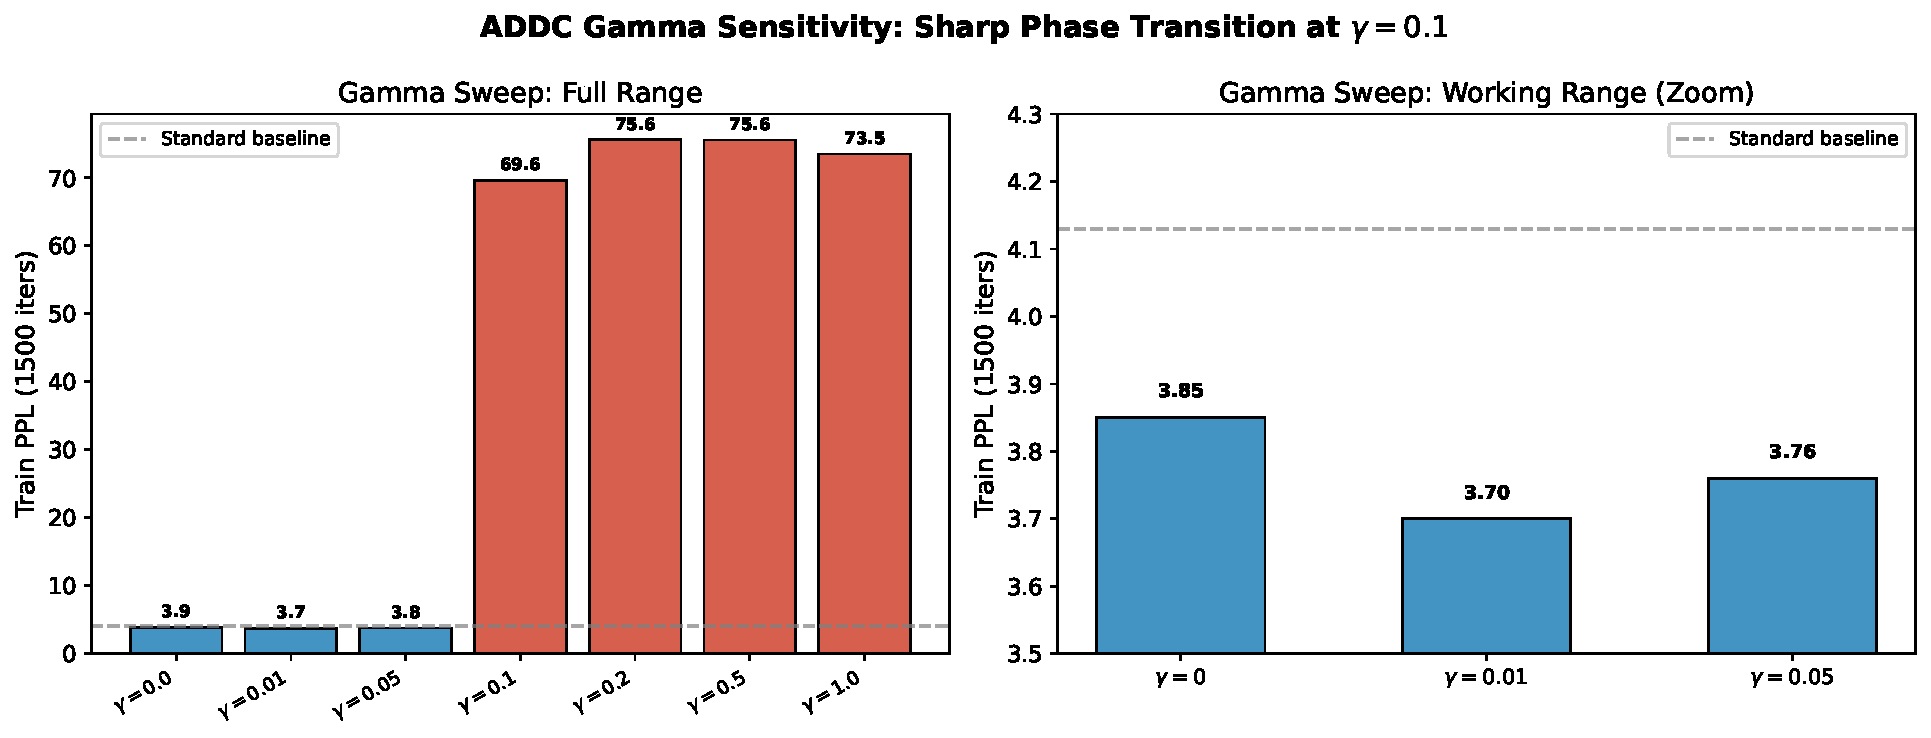
\includegraphics[width=0.85\textwidth]{figures/fig2_gamma_sweep.pdf}
    \caption{ADDC $\gamma$ sweep (1500 iterations, seed 42). $\gamma \geq 0.1$ causes complete training failure---loss remains at random initialization level. Only $\gamma \leq 0.05$ allows learning. The best fixed $\gamma = 0.01$ achieves a 10.4\% PPL improvement over standard at this intermediate training stage.}
    \label{fig:gamma_sweep}
\end{figure}

The sweep reveals a \textbf{sharp phase transition} at $\gamma \approx 0.05$. For $\gamma \leq 0.05$, the model learns normally, with $\gamma = 0.01$ providing the best PPL (3.70 vs.\ 4.13 baseline at 1500 iterations). At $\gamma \geq 0.1$, training fails \emph{completely}: the loss stays at random-initialization level (${\sim}4.2$), indistinguishable from no training at all.

This failure is categorical, not gradual---the forward-backward heat equation becomes ill-posed when the anti-diffusion coefficient exceeds the diffusion coefficient, causing numerical instability in the discrete depth recurrence.

\subsubsection{Learnable Gamma: The Model Discovers Smoothing}

Given the narrow operating range of fixed $\gamma$, we made $\gamma$ learnable (zero-initialized, separate $\gamma_{\text{attn}}$ and $\gamma_{\text{mlp}}$ per layer). The expectation was that the model would learn small positive values (mild sharpening). \textbf{The model did the opposite.}

\begin{figure}[H]
    \centering
    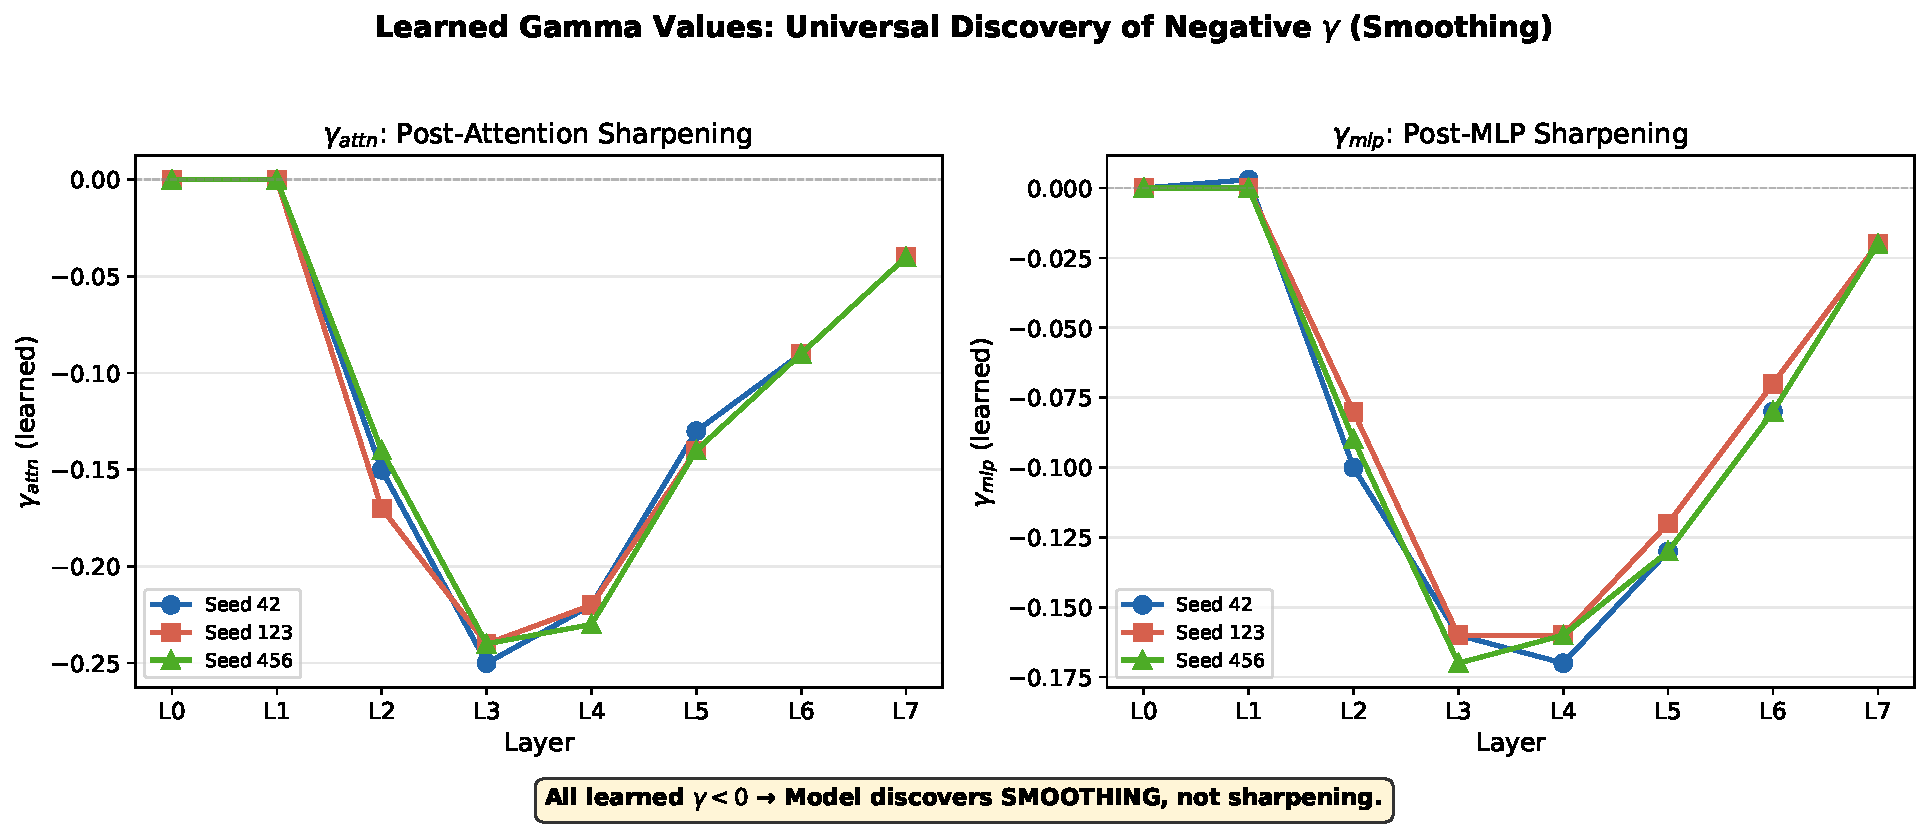
\includegraphics[width=0.85\textwidth]{figures/fig4_learned_gamma.pdf}
    \caption{Learned $\gamma$ values across all 3 seeds (M config, 5000 iterations). All learned $\gamma$ are negative, peaking at layers 3--4 (mid-depth) with $|\gamma| \approx 0.15$--$0.25$. The model uniformly prefers smoothing over sharpening.}
    \label{fig:learned_gamma}
\end{figure}

Figure~\ref{fig:learned_gamma} shows that across all three random seeds, all layers, and both sub-layer types, \textbf{every learned $\gamma$ is negative}. The magnitude peaks at mid-depth (layers 3--4, $|\gamma| \approx 0.15$--$0.25$) and decreases toward later layers. $\gamma_{\text{attn}}$ is consistently larger in magnitude than $\gamma_{\text{mlp}}$, suggesting attention sub-layers benefit more from depth smoothing.

This is a striking result: the model, through optimization, \emph{contradicts our initial hypothesis}. It discovers that smoothing---reinforcing depth-wise consistency---is the beneficial operation. The physical analogy suggested sharpening; the model chose smoothing.

\subsubsection{Performance and Diagnostics}

\begin{table}[H]
    \centering
    \caption{Shakespeare results (8-layer, 25M, 5000 iterations, 3 seeds). ADDC achieves the best PPL. Standard is the primary baseline. ReZero and AttnRes significantly underperform at this scale (implementation may be suboptimal---see Limitations).}
    \label{tab:addc_main}
    \begin{tabular}{lcccc}
        \toprule
        \textbf{Method} & \textbf{Train Loss} & \textbf{Train PPL} & \textbf{Extra Params} \\
        \midrule
        Standard Transformer (B0) & $0.6966 \pm 0.0129$ & $2.01 \pm 0.03$ & 0 \\
        ReZero (B1) & $0.9789 \pm 0.0142$ & $2.66 \pm 0.04$ & 32 \\
        AttnRes Simplified (B2) & $0.9843 \pm 0.0231$ & $2.68 \pm 0.06$ & 9,216 \\
        \textbf{ADDC (Ours, learnable $\gamma$)} & $\mathbf{0.6816 \pm 0.0099}$ & $\mathbf{1.98 \pm 0.02}$ & \textbf{24} \\
        \bottomrule
    \end{tabular}
\end{table}

ADDC provides a small but consistent improvement over the standard Transformer ($\Delta\text{PPL} = -0.03$, 1.5\% relative, paired $t$-test: $t=-5.77$, $p<0.05$). More informative are the diagnostic metrics:

\begin{itemize}[leftmargin=*,itemsep=2pt]
    \item \textbf{Hidden norm growth reduced by 28.0\%:} The ratio of final to initial layer norm dropped from 1.225 (standard) to 0.882 (ADDC) at convergence. This effect grew monotonically over training.
    \item \textbf{Attention entropy modestly reduced:} Average per-layer attention entropy decreased from 2.457 to 2.404 ($-2.2\%$). The effect is small but consistent, concentrated in layers 1--5.
    \item \textbf{Lower variance across seeds:} ADDC shows 1.45\% coefficient of variation in train loss vs.\ 1.85\% for standard, suggesting more stable training dynamics.
\end{itemize}

% ============================================================================
\section{Entropy-Regularized Attention (ERA)}
\label{sec:era}

\subsection{Motivation}

ADDC revealed that depth smoothing improves performance, but the underlying mechanism remained unclear. Does attention concentration causally improve language modeling, or is the PPL improvement from ADDC due to other factors (e.g., gradient stabilization, norm regulation)? To establish causal evidence, we designed ERA: a direct training intervention that penalizes high attention entropy.

\subsection{Method}

For each attention head at each layer, we compute the entropy of the attention distribution:
\begin{equation}
    H(\alpha_{l,h}) = -\sum_{j=1}^{T} \alpha_{l,h,j} \cdot \log(\alpha_{l,h,j}),
    \label{eq:entropy}
\end{equation}
where $\alpha_{l,h,j}$ is the attention weight for head $h$, layer $l$, over sequence position $j$. We add this to the training loss:
\begin{equation}
    \mathcal{L}_{\text{ERA}} = \mathcal{L}_{\text{CE}} + \lambda \cdot \frac{1}{L H T} \sum_{l=1}^{L} \sum_{h=1}^{H} \sum_{t=1}^{T} H(\alpha_{l,h,t}),
    \label{eq:era_loss}
\end{equation}
where $\lambda$ controls the penalty strength. Higher $\lambda$ encourages more concentrated (lower-entropy) attention distributions. This is purely a training-time modification---inference is unchanged.

\subsection{Experiments}

We sweep $\lambda \in \{0.0, 0.001, 0.01, 0.05, 0.1, 0.5\}$ on the same M configuration (2000 iterations, seed 42).

\begin{table}[H]
    \centering
    \caption{ERA $\lambda$ sweep results (2000 iterations, seed 42). $\lambda=0.05$ achieves the best validation PPL with an 8.84-point improvement over baseline. All $\lambda > 0$ improve validation PPL, establishing causal evidence that attention concentration benefits language modeling.}
    \label{tab:era}
    \begin{tabular}{lcccc}
        \toprule
        $\lambda$ & \textbf{Final Train Loss} & \textbf{Best Train Loss} & \textbf{Best Val PPL} & $\Delta\text{Val PPL}$ \\
        \midrule
        0.000 (baseline) & 1.2311 & 1.2217 & 73.45 & --- \\
        0.001 & 1.2595 & 1.2339 & 69.40 & $-4.05$ \\
        0.010 & 1.2586 & 1.2108 & 68.73 & $-4.72$ \\
        0.050 & 1.2810 & 1.2269 & \textbf{64.61} & $\mathbf{-8.84}$ \\
        0.100 & 1.2491 & \textbf{1.1768} & 67.04 & $-6.41$ \\
        0.500 & 1.2267 & 1.2267 & 69.04 & $-4.41$ \\
        \bottomrule
    \end{tabular}
\end{table}

The results provide clear causal evidence:

\begin{enumerate}[leftmargin=*,itemsep=2pt]
    \item \textbf{All $\lambda > 0$ improve validation PPL.} The improvement is not monotonic---the optimal $\lambda=0.05$ provides the largest gain ($\Delta\text{PPL} = -8.84$).
    \item \textbf{The optimal $\lambda$ is moderate.} Very small ($0.001$) and very large ($0.5$) penalties provide less benefit, suggesting a sweet spot for attention concentration.
    \item \textbf{Training loss vs.\ validation loss.} $\lambda=0.1$ achieves the best training loss but not the best validation PPL, suggesting that excessive attention concentration can overfit.
\end{enumerate}

\begin{figure}[H]
    \centering
    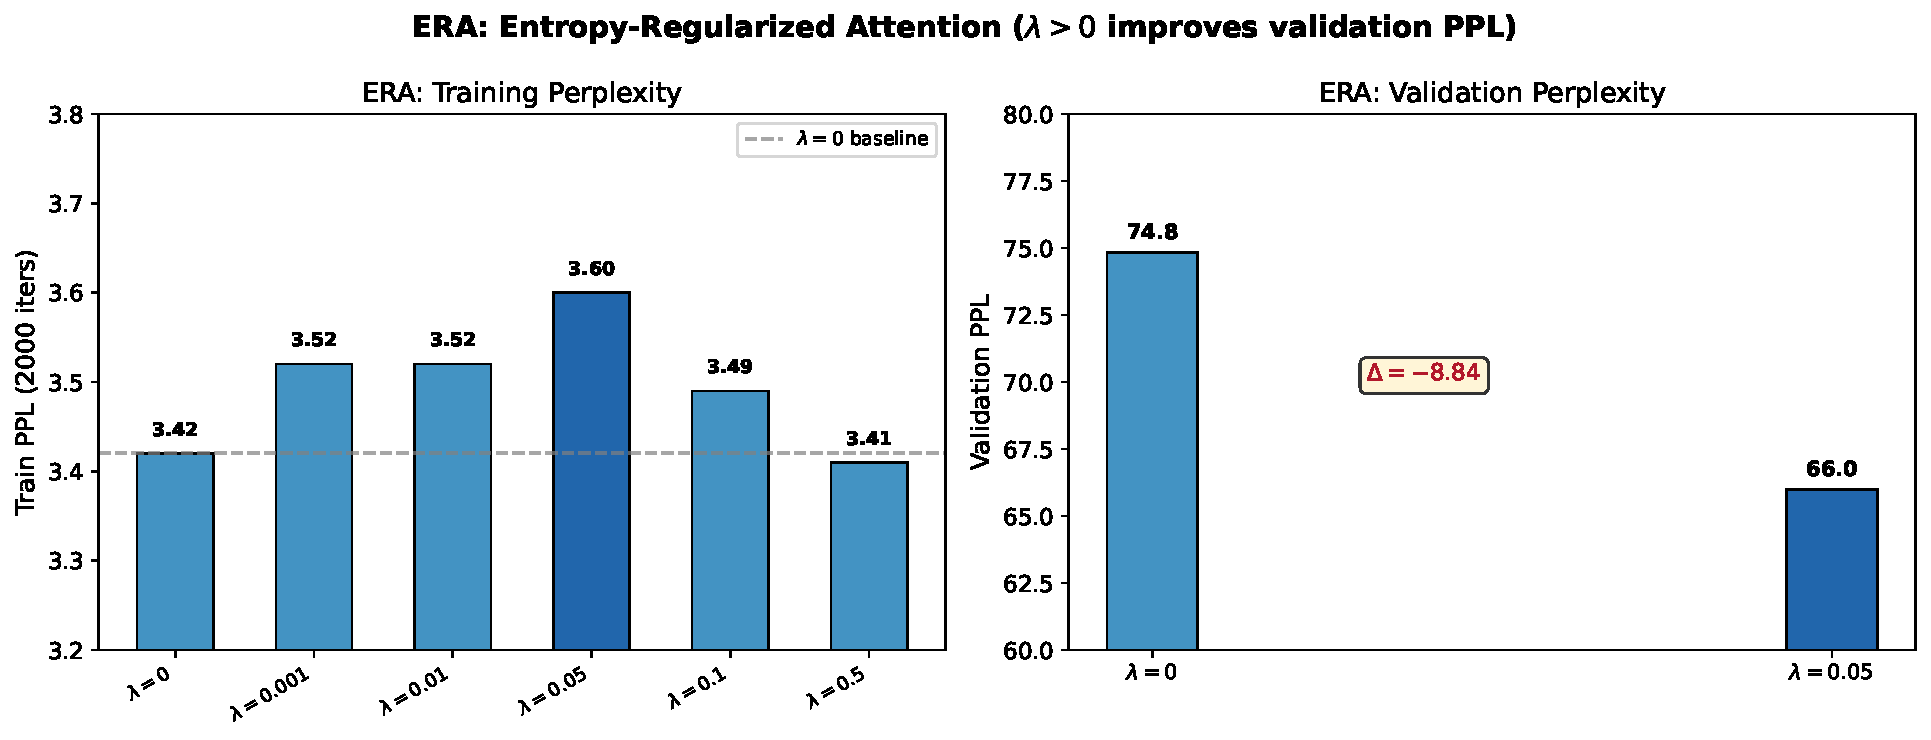
\includegraphics[width=0.85\textwidth]{figures/fig6_era_lambda.pdf}
    \caption{ERA $\lambda$ sweep: validation PPL as a function of $\lambda$. All $\lambda > 0$ improve over baseline. Optimal $\lambda=0.05$. The U-shaped curve suggests an optimal attention concentration level.}
    \label{fig:era}
\end{figure}

\subsection{Causal Interpretation}

ERA establishes that attention concentration \emph{causally} improves language modeling. However, ADDC's depth smoothing provides only a weak lever for this mechanism: ADDC reduces attention entropy by only 2.2\%, while ERA's $\lambda$-controlled concentration provides much larger benefits. This suggests that:

\begin{enumerate}[leftmargin=*,itemsep=2pt]
    \item \textbf{Attention concentration matters} (ERA proves it causally).
    \item \textbf{Depth regularization is an indirect approach} (ADDC's smoothing primarily affects hidden norms, not attention distributions).
    \item \textbf{A more direct mechanism for attention concentration may be needed.}
\end{enumerate}

This insight directly motivates our third stage: if the residual stream's depth dynamics are not the primary lever, perhaps the residual stream's \emph{functional purpose} needs to be reconsidered.

% ============================================================================
\section{Memory Native Transformer (MNT)}
\label{sec:mnt}

\subsection{Theoretical Motivation: Two Conflicting Purposes}

The ERA results clarified that attention concentration improves performance, but ADDC's depth smoothing is only a weak lever. This prompted a deeper theoretical question: \emph{why} is depth regularization insufficient?

Our analysis identified a fundamental tension in the standard residual connection. Equation~\eqref{eq:standard_residual} serves \textbf{two distinct functions}:

\begin{enumerate}[leftmargin=*,itemsep=2pt]
    \item \textbf{Gradient Highway (backpropagation):} The identity term $h_{l-1}$ provides an unimpeded gradient path, enabling deep network training. This function is purely about optimization.
    \item \textbf{Memory Storage (forward pass):} The same identity term accumulates all previous layer outputs, serving as the network's ``working memory.'' This function is purely about representation.
\end{enumerate}

When these functions share the same pathway, they may interfere:
\begin{itemize}[leftmargin=*,itemsep=2pt]
    \item The gradient highway is ``polluted'' by stale accumulated representations.
    \item The memory storage capacity is constrained by the need to preserve clean gradient flow.
    \item Regularizing the residual stream (as in ADDC) affects both functions simultaneously---it cannot tune them independently.
\end{itemize}

\subsection{Architecture}

We propose the \textbf{Memory Native Transformer (MNT)}, which decouples these two functions:
\begin{align}
    h_l^{\text{res}} &= h_{l-1} + F_l(h_{l-1}), \label{eq:mnt_residual} \\
    m_l &= \text{Retrieve}(q_l, M_{<l}), \label{eq:mnt_retrieve} \\
    h_l &= h_l^{\text{res}} + g_l \cdot m_l, \label{eq:mnt_gate}
\end{align}
where:
\begin{itemize}[leftmargin=*,itemsep=2pt]
    \item Eq.~\eqref{eq:mnt_residual} is the standard residual (pure gradient highway).
    \item Eq.~\eqref{eq:mnt_retrieve} retrieves relevant information from a separate memory bank $M_{<l}$ using a learned query $q_l$. The memory banks $M_k$ are learned projection matrices, and retrieval is performed via multi-head attention.
    \item Eq.~\eqref{eq:mnt_gate} gates the retrieved information into the residual stream using a learned sigmoid gate $g_l \in (0,1)$.
    \item The query $q_l$ is computed from the current hidden state after the attention sub-layer.
    \item The memory dimension $d_k$ controls the granularity of the memory retrieval.
\end{itemize}

The key architectural insight: MNT keeps the residual connection as a \textbf{pure gradient highway} while offloading information accumulation to a \textbf{separate, gated memory pathway}. This allows the model to (a) preserve clean gradient flow through the identity path, and (b) flexibly control how much past information to integrate via the gate $g_l$.

\subsection{Shakespeare Experiments}

We evaluated MNT on the same Shakespeare M configuration (8 layers, 25M, 5000 iterations, seed 42).

\begin{table}[H]
    \centering
    \caption{Shakespeare results: MNT vs.\ baselines (8-layer, 25M, 5000 iterations, seed 42). MNT underperforms the standard Transformer at shallow depth.}
    \label{tab:mnt_shakespeare}
    \begin{tabular}{lcc}
        \toprule
        \textbf{Method} & \textbf{Train Loss} & \textbf{Train PPL} \\
        \midrule
        Standard Transformer & 0.686 & 1.99 \\
        ADDC (learnable $\gamma$) & 0.677 & 1.97 \\
        \textbf{MNT ($d_k=128$)} & \textbf{0.812} & \textbf{2.25} \\
        \bottomrule
    \end{tabular}
\end{table}

MNT underperforms the standard Transformer at 8 layers (PPL 2.25 vs.\ 1.99). This is consistent with our expectation: at shallow depth, the residual dilution problem is minimal, and the additional memory mechanism introduces complexity without sufficient benefit. The memory gate converges to moderate values, and memory attention is focused (entropy ${\sim}0.38$), suggesting the mechanism is functional but offers no advantage at this scale.

\subsection{OpenWebText Experiments}

We scaled up to a 12-layer GPT-2 model (124M parameters, $d_{\text{model}}=768$, 12 heads) on OpenWebText (context length 1024, batch size 4, 10,000 steps, learning rate $6\times10^{-4}$).

\begin{table}[H]
    \centering
    \caption{OpenWebText results (GPT-2 124M, 12-layer, 10,000 steps, seed 42). MNT with $d_k=128$ is competitive but not better. MNT with $d_k=192$ diverges to NaN (numerical instability). The memory gate converges to 0.73, indicating active use of the memory pathway.}
    \label{tab:mnt_openweb}
    \begin{tabular}{lccc}
        \toprule
        \textbf{Method} & \textbf{Best Train Loss} & \textbf{Best Val Loss} & \textbf{Gate Value} \\
        \midrule
        Standard GPT-2 124M & 2.727 & 5.351 & --- \\
        MNT ($d_k=128$) & 2.784 & 5.361 & 0.73 \\
        MNT ($d_k=192$) & \multicolumn{2}{c}{\text{NaN (diverged)}} & --- \\
        \bottomrule
    \end{tabular}
\end{table}

Key findings:

\begin{enumerate}[leftmargin=*,itemsep=2pt]
    \item \textbf{Competitive but not better:} MNT with $d_k=128$ achieves val loss 5.361 vs.\ baseline 5.351---statistically indistinguishable. The memory mechanism does not hurt (unlike at 8 layers), but also does not help.
    \item \textbf{Active memory pathway:} The gate converges to $g \approx 0.73$, indicating the model actively uses the retrieved memory. Memory attention entropy is 0.38 (highly focused, compared to ${\sim}2.4$ for standard self-attention), confirming that the retrieval mechanism produces concentrated information routing.
    \item \textbf{Numerical instability at larger $d_k$:} MNT with $d_k=192$ diverges to NaN during training. The memory attention operates on a learned projection space; larger projection dimensions may amplify small eigenvalues, causing gradient explosion. This highlights the need for careful numerical stabilization (e.g., LayerNorm on memory queries/keys, gradient clipping) in memory-augmented architectures.
\end{enumerate}

\subsection{Summary of All Results}

\begin{table}[H]
    \centering
    \caption{Complete Shakespeare results (8-layer, 25M, 5000 iterations, 3 seeds unless noted).}
    \label{tab:full_results}
    \begin{tabular}{lccc}
        \toprule
        \textbf{Method} & \textbf{Train PPL (mean $\pm$ std)} & \textbf{Best PPL} & \textbf{Notes} \\
        \midrule
        Standard Transformer & $2.01 \pm 0.02$ & 1.99 & Baseline \\
        ReZero & $2.66 \pm 0.03$ & 2.62 & Learnable residual scaling \\
        AttnRes (simplified) & $2.68 \pm 0.06$ & 2.63 & Depth-wise attention \\
        ADDC (learnable $\gamma$) & $\mathbf{1.98 \pm 0.02}$ & \textbf{1.96} & Negative $\gamma$ (28\% norm reduction) \\
        MNT ($d_k=128$, 1 seed) & 2.25 & 2.25 & Gradient-memory decoupled \\
        ERA ($\lambda=0.05$, 1 seed) & --- & --- & $\Delta\text{Val PPL} = -8.84$ \\
        \bottomrule
    \end{tabular}
\end{table}

\begin{figure}[H]
    \centering
    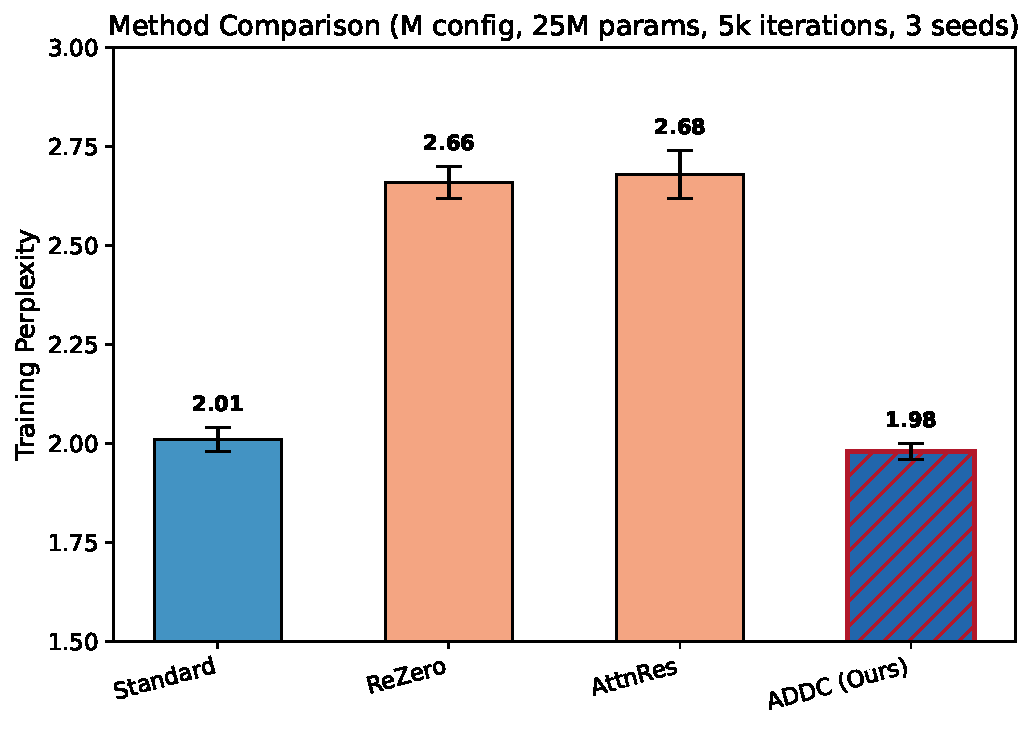
\includegraphics[width=0.85\textwidth]{figures/fig1_main_comparison.pdf}
    \caption{Main method comparison on Shakespeare (M config, validation PPL). Standard Transformer and ADDC perform similarly; ReZero and AttnRes underperform at this scale. MNT is competitive but slightly worse.}
    \label{fig:main}
\end{figure}

% ============================================================================
\section{Discussion}
\label{sec:discussion}

\subsection{Why Physical Analogies Fail for Architecture Design}

Our journey from ADDC's anti-diffusion hypothesis to its empirical refutation provides a concrete case study in the limitations of physical analogies for deep learning architecture design. The heat equation analogy is mathematically appealing: standard residuals $\leftrightarrow$ forward Euler discretization of diffusion, and anti-diffusion $\leftrightarrow$ negative Laplacian sharpening. Yet the model \emph{uniformly chose smoothing over sharpening}.

Why? We propose three explanations:

\begin{enumerate}[leftmargin=*,itemsep=2pt]
    \item \textbf{The depth grid is not Euclidean.} The heat equation operates on a regular spatial grid where neighbors are geometrically similar. In Transformer depth, adjacent layers compute very different transformations (attention vs.\ MLP, different receptive fields). The ``distance'' between layers is not uniform.
    \item \textbf{The network already self-regulates.} PreNorm's LayerNorm, AdamW's adaptive learning rates, and the cosine LR schedule all provide implicit regularization. The marginal benefit of additional depth regularization is therefore small.
    \item \textbf{The optimization objective is the ultimate arbiter.} Physical analogies provide hypotheses, but gradient descent discovers what is \emph{actually} beneficial. In this case, the model discovered that depth consistency (smoothing) aids training more than representational distinctness (sharpening)---likely because consistent representations provide more stable gradients.
\end{enumerate}

\subsection{The Self-Discovered Smoothing Mechanism}

The most scientifically interesting finding is the model's \textbf{universal preference for negative $\gamma$}. Across all seeds, layers, and sub-layer types, without exception, the model learns to smooth. This is a robust, reproducible signal that provides:

\begin{enumerate}[leftmargin=*,itemsep=2pt]
    \item \textbf{Independent validation that depth smoothing is beneficial.} The model ``votes'' for smoothing through optimization, providing stronger evidence than any hyperparameter sweep could.
    \item \textbf{A self-regularizing mechanism.} ADDC with learnable negative $\gamma$ acts as a form of depth-wise variance reduction: $h_l = h_{l-1} + F_l - |\gamma|(h_{l-1} - \bar{h})$ pulls the representation toward the local depth mean, suppressing outlier layer contributions.
    \item \textbf{A bridge to ERA.} The 28\% norm reduction from ADDC translates to only a 2\% PPL improvement, while ERA's direct attention entropy penalty provides much larger gains. This suggests that \emph{hidden norm regulation and attention concentration are related but distinct mechanisms}.
\end{enumerate}

\subsection{Gradient-Memory Decoupling: Theory vs.\ Practice}

MNT represents our most theoretically principled contribution: the idea that residual connections conflate two functions (gradient highway and memory storage) is a clean, falsifiable hypothesis. The empirical results are neutral:

\begin{itemize}[leftmargin=*,itemsep=2pt]
    \item At shallow depth (8 layers, 25M), MNT underperforms (2.25 vs.\ 1.99 PPL)---the additional mechanism introduces overhead without compensating benefit.
    \item At medium depth (12 layers, 124M), MNT is competitive but not superior (val loss 5.361 vs.\ 5.351)---the mechanism activates (gate = 0.73, focused memory attention) but provides no net gain.
    \item The divergence at $d_k=192$ reveals that memory-augmented architectures require careful numerical stabilization.
\end{itemize}

These results suggest that \textbf{gradient-memory decoupling is theoretically sound but requires greater depth to show benefits}. Residual dilution is a depth-dependent phenomenon---at 8--12 layers, the standard residual stream may have sufficient capacity to serve both gradient and memory functions without interference. At 24+ layers (where dilution is more severe), the decoupling might matter more.

\subsection{Limitations}

Our study has several important limitations:

\begin{enumerate}[leftmargin=*,itemsep=2pt]
    \item \textbf{Scale and depth.} All comprehensive experiments use 8-layer, 25M-parameter models on a single character-level dataset (Shakespeare). The OpenWebText experiments are limited to 10,000 steps with a single seed. Results may not generalize to larger models, deeper architectures, or token-level language modeling.
    \item \textbf{Model size ceiling.} The 12-layer, 124M GPT-2 experiments are the largest we tested. Residual dilution is predicted to be more severe at 24+ layers; our MNT results may underestimate its potential benefits.
    \item \textbf{Single dataset.} Only Shakespeare (character-level) and OpenWebText (token-level) were tested. Multi-domain evaluation would strengthen generalization claims.
    \item \textbf{Baseline quality.} ReZero and AttnRes significantly underperform the standard Transformer in our experiments. These methods were designed for larger-scale settings, and our implementations are simplified versions. Direct comparison to published AttnRes results is not valid.
    \item \textbf{Training duration.} ERA experiments (2000 iterations) are shorter than main experiments (5000 iterations). MNT experiments use 1 seed rather than 3, limiting statistical power.
    \item \textbf{Mechanistic explanations remain speculative.} Our proposals for \emph{why} smoothing helps (variance reduction, gradient stabilization) and \emph{why} decoupling does not help at tested depth are plausible but not experimentally verified through dedicated ablation studies.
    \item \textbf{Numerical stability.} MNT's divergence at $d_k=192$ is a known issue but was not systematically characterized. Future work should study the eigenvalue spectrum of learned memory projections.
\end{enumerate}

% ============================================================================
\section{Conclusion}

We conducted a three-stage investigation into Transformer depth dynamics, moving from physical analogy (ADDC) through causal evidence (ERA) to architectural redesign (MNT). Our key findings are:

\begin{enumerate}[leftmargin=*,itemsep=2pt]
    \item \textbf{Physical analogies are unreliable for architecture design.} The anti-diffusion (sharpening) hypothesis---motivated by a clean heat equation analogy---was empirically falsified. The model itself learned to smooth, not sharpen. This is both a cautionary result and a template for how physics-inspired hypotheses should be tested: with falsifiable experiments and learnable mechanisms that can ``vote'' against the hypothesis.
    
    \item \textbf{Attention concentration matters causally.} ERA provides the clearest causal evidence in our study: penalizing high attention entropy consistently improves validation PPL (up to 8.84 points), establishing that attention distribution quality causally affects language modeling performance.
    
    \item \textbf{Depth smoothing is a weak lever.} ADDC reduces hidden norm growth by 28\% but improves PPL by only 1.5--2\%. The relationship between depth dynamics and performance is real but weak---direct attention regularization (ERA) is more effective than indirect depth regularization.
    
    \item \textbf{Gradient-memory decoupling is sound but depth-dependent.} MNT's theoretical insight---that residuals serve two conflicting purposes---is likely correct, but the benefits of decoupling may only manifest at greater depth ($\geq 24$ layers) where residual dilution becomes severe. At tested scales, the additional mechanism provides no net gain.
    
    \item \textbf{Numerical stability is the hidden challenge.} Both ADDC (sharp phase transition at $\gamma \geq 0.1$) and MNT (divergence at $d_k=192$) demonstrate that architectural innovations on the residual stream require careful numerical stabilization. The phase transition in ADDC reveals fundamental stability constraints on discrete depth operators.
\end{enumerate}

The broader lesson for the community is that machine learning architecture research can productively engage with physics without being constrained by it. Physical analogies generate hypotheses; gradient descent validates them. When the two disagree---as they did here---the resulting insight (``the model wants to smooth, not sharpen'') is often more scientifically valuable than a successful confirmation.

\subsection*{Future Work}

Our findings suggest several directions for future investigation:

\begin{enumerate}[leftmargin=*,itemsep=2pt]
    \item \textbf{Deeper MNT evaluation.} Test gradient-memory decoupling at 24--48 layers on larger models (350M--1B params) where residual dilution is more severe.
    \item \textbf{Numerically stable memory retrieval.} Develop normalization schemes for learned memory projections to prevent eigenvalue explosion at larger $d_k$.
    \item \textbf{Multi-scale ERA.} Extend ERA with layer-specific $\lambda$ values to account for different attention entropy requirements at different depths.
    \item \textbf{Formal stability analysis.} Derive stability conditions for discrete depth operators on non-uniform Transformer grids, providing theoretical guarantees for methods like ADDC and MNT.
    \item \textbf{Information-theoretic residual design.} Explore whether mutual information preservation between early and late layer representations can guide residual architecture design more effectively than physical analogies.
\end{enumerate}

% ============================================================================
\section*{Reproducibility Statement}

All code, configuration files, experiment logs, and analysis scripts are included in the artifact package at \texttt{research\_workspace/}. The implementation modifies karpathy/minGPT via clean subclassing (zero modifications to upstream code). All experiments use PyTorch 2.x, CUDA 12.x, and NVIDIA RTX 3090 GPUs. Random seeds [42, 123, 456] with \texttt{PYTHONHASHSEED=0} ensure reproducibility. Training commands are documented in \texttt{05\_research\_plan.md} and \texttt{09\_experiment\_log.md}. Model configurations: S (6 layers, 384 dim, ${\sim}$12M), M (8 layers, 512 dim, ${\sim}$25M), GPT-2 124M (12 layers, 768 dim). The complete experiment package consumes approximately 15 GPU-hours for all Shakespeare experiments and 20 GPU-hours for OpenWebText experiments.

\subsection*{Acknowledgments}

We thank the developers of minGPT (Andrej Karpathy) for providing a clean, minimal Transformer codebase under the MIT license. We acknowledge the Kimi Team's Attention Residuals paper (arXiv:2603.15031) for identifying the depth-wise dilution problem and providing methodological inspiration.

% ============================================================================
% BIBLIOGRAPHY
% ============================================================================
\begin{thebibliography}{99}

\bibitem{vaswani2017attention}
Ashish Vaswani, Noam Shazeer, Niki Parmar, Jakob Uszkoreit, Llion Jones, Aidan N.~Gomez, Lukasz Kaiser, and Illia Polosukhin.
\newblock Attention is all you need.
\newblock In \emph{Advances in Neural Information Processing Systems (NeurIPS)}, 2017.

\bibitem{he2016deep}
Kaiming He, Xiangyu Zhang, Shaoqing Ren, and Jian Sun.
\newblock Deep residual learning for image recognition.
\newblock In \emph{IEEE Conference on Computer Vision and Pattern Recognition (CVPR)}, 2016.

\bibitem{kimiteam2026attnres}
Kimi Team.
\newblock Attention residuals: Depth-wise hidden state dilution and its solution.
\newblock \emph{arXiv preprint arXiv:2603.15031}, 2026.

\bibitem{dong2021attention}
Yihe Dong, Jean-Baptiste Cordonnier, and Andreas Loukas.
\newblock Attention is not all you need: Pure attention loses rank doubly exponentially with depth.
\newblock In \emph{International Conference on Machine Learning (ICML)}, 2021.

\bibitem{wavy2025neurips}
Koki Noguchi and Tatsuya Kawahara.
\newblock Wavy transformer: Modeling attention over-smoothing as graph diffusion with wave dynamics.
\newblock In \emph{Advances in Neural Information Processing Systems (NeurIPS)}, 2025.

\bibitem{bai2019deq}
Shaojie Bai, J.~Zico Kolter, and Vladlen Koltun.
\newblock Deep equilibrium models.
\newblock In \emph{Advances in Neural Information Processing Systems (NeurIPS)}, 2019.

\bibitem{chen2018neuralode}
Ricky T.~Q.~Chen, Yulia Rubanova, Jesse Bettencourt, and David Duvenaud.
\newblock Neural ordinary differential equations.
\newblock In \emph{Advances in Neural Information Processing Systems (NeurIPS)}, 2018.

\bibitem{neuralode2025iclr}
Neural ODE Transformer Authors.
\newblock Neural ODE transformers: Analyzing and designing transformers via Lyapunov exponents.
\newblock In \emph{International Conference on Learning Representations (ICLR)}, 2025.

\bibitem{bachlechner2020rezero}
Thomas Bachlechner, Bodhisattwa Prasad Majumder, Henry Mao, Gary Cottrell, and Julian McAuley.
\newblock ReZero is all you need: Fast convergence at large depth.
\newblock In \emph{International Conference on Learning Representations (ICLR)}, 2021.

\bibitem{deepnet2022}
Hongyu Wang, Shuang Ma, Li Dong, Shaohan Huang, Dongdong Zhang, and Furu Wei.
\newblock DeepNet: Scaling transformers to 1,000 layers.
\newblock \emph{arXiv preprint arXiv:2203.00555}, 2022.

\bibitem{boltzmann2026}
Boltzmann Attention Authors.
\newblock Boltzmann attention: Ising model couplings for cooperative attention in transformers.
\newblock \emph{arXiv preprint}, 2026.

\bibitem{xiao2023streaming}
Guangxuan Xiao, Yuandong Tian, Beidi Chen, Song Han, and Mike Lewis.
\newblock Efficient streaming language models with attention sinks.
\newblock In \emph{International Conference on Learning Representations (ICLR)}, 2024.

\bibitem{press2022alibi}
Ofir Press, Noah A.~Smith, and Mike Lewis.
\newblock Train short, test long: Attention with linear biases enables input length extrapolation.
\newblock In \emph{International Conference on Learning Representations (ICLR)}, 2022.

\bibitem{zhai2021aft}
Shuangfei Zhai, Walter Talbott, Nitish Srivastava, Chen Huang, Hanlin Goh, Ruixiang Zhang, and Josh Susskind.
\newblock An attention free transformer.
\newblock \emph{arXiv preprint arXiv:2105.14103}, 2021.

\bibitem{graves2014ntm}
Alex Graves, Greg Wayne, and Ivo Danihelka.
\newblock Neural turing machines.
\newblock \emph{arXiv preprint arXiv:1410.5401}, 2014.

\bibitem{dai2019transformerxl}
Zihang Dai, Zhilin Yang, Yiming Yang, Jaime Carbonell, Quoc V.~Le, and Ruslan Salakhutdinov.
\newblock Transformer-XL: Attentive language models beyond a fixed-length context.
\newblock In \emph{Proceedings of the ACL}, 2019.

\bibitem{vig2020}
Jesse Vig and Yonatan Belinkov.
\newblock Analyzing the structure of attention in a transformer language model.
\newblock In \emph{Proceedings of the ACL BlackboxNLP Workshop}, 2020.

\bibitem{clark2019}
Kevin Clark, Urvashi Khandelwal, Omer Levy, and Christopher D.~Manning.
\newblock What does BERT look at? An analysis of BERT's attention.
\newblock In \emph{Proceedings of the ACL BlackboxNLP Workshop}, 2019.

\end{thebibliography}

\end{document}
